\clearpage
\item \points{40} {\bf Linear Classifiers (logistic regression and GDA)}

In this problem, we cover two probabilistic linear classifiers we have
covered in class so far. First, a discriminative linear classifier: logistic
regression. Second, a generative linear classifier: Gaussian discriminant
analysis (GDA). Both the algorithms find a linear decision boundary that
separates the data into two classes, but make different assumptions. Our goal
in this problem is to get a deeper understanding of the similarities and
differences (and, strengths and weaknesses) of these two algorithms.

For this problem, we will consider two datasets, provided in the following
files:
\begin{enumerate}[label=\roman*.]
	\item \url{data/ds1_{train,valid}.csv}
	\item \url{data/ds2_{train,valid}.csv}
\end{enumerate}
Each file contains $m$ examples, one example $(x^{(i)}, y^{(i)})$ per row.
In particular, the $i$-th row contains columns $x^{(i)}_0\in\Re$,
$x^{(i)}_1\in\Re$, and $y^{(i)}\in\{0, 1\}$. In the subproblems that follow, we
will investigate using logistic regression and Gaussian discriminant analysis
(GDA) to perform binary classification on these two datasets.

\begin{enumerate}
	\item \subquestionpoints{10}
In lecture we saw the average empirical loss for logistic regression:
\begin{equation*}
	J(\theta)
	= -\frac{1}{m} \sum_{i=1}^m y^{(i)}\log(h_{\theta}(x^{(i)}))
		+  (1 - y^{(i)})\log(1 - h_{\theta}(x^{(i)})),
\end{equation*}
where $y^{(i)} \in \{0, 1\}$, $h_\theta(x) = g(\theta^T x)$ and
$g(z) = 1 / (1 + e^{-z})$.

Find the Hessian $H$ of this function, and show that for any vector $z$, it
holds true that
%
\begin{equation*}
    z^T H z \ge 0.
\end{equation*}
%
{\bf Hint:} You may want to start by showing that
$\sum_i\sum_j z_i x_i x_j z_j = (x^Tz)^2 \geq 0$. Recall also that
$g'(z) = g(z)(1-g(z))$.

{\bf Remark:} This is one of the standard ways of showing that the matrix $H$
is positive semi-definite, written ``$H \succeq 0$.''  This implies that $J$ is
convex, and has no local minima other than the global one. If you have some
other way of showing $H \succeq 0$, you're also welcome to use your method
instead of the one above.

\ifnum\solutions=1 {
  \begin{answer}
\newline
First calculate first partial derivative:
\begin{equation*}
	\begin{aligned}
		\frac{ \partial J ( \theta )}{\partial \theta _j} &= -\frac{1}{m} \sum_{i=1}^m y^{(i)} \frac{1}{h_\theta(x^{(i)})}\frac{\partial}{\partial \theta _j}h_\theta (x^{(i)}) + (1-y^{(i)}) \frac{1}{1-h_\theta(x^{(i)})}\frac{\partial}{\partial \theta _j}(1-h_\theta(x^{(i)}) ) \\
		&= -\frac{1}{m} \sum_{i=1}^m y^{(i)} \frac{1}{g(\theta ^T x^{(i)})}\frac{\partial}{\partial \theta _j}h_\theta (x^{(i)}) + (1-y^{(i)}) \frac{1}{1-g(\theta ^T x^{(i)})}\frac{\partial}{\partial \theta _j}(1-g(\theta ^T x^{(i)}) ) \\
		&= -\frac{1}{m} \sum_{i=1}^{m}  y^{(i)} \left[1 - g(\theta^T x^{(i)})\right]x^{(i)}_j - (1 - y^{(i)}) g(\theta^T x^{(i)})x^{(i)}_j  \\
		&= \frac{1}{m} \sum_{i=1}^{m} \left[ g(\theta^T x^{(i)}) - y^{(i)} \right]x^{(i)}_j \\
	\end{aligned}
\end{equation*}
Therefore, we have the gradient:
\begin{equation*}
		\nabla _\theta J(\theta) = \frac{1}{m} X^T (g(X \theta) - Y )
\end{equation*}

Then calculate second partial derivative:

\begin{equation*}
		H_{jk} = \frac{\partial^2 J(\theta)}{\partial \theta_j \partial \theta_k} = \frac{1}{m} \sum_{i=1}^m g(\theta ^ T x^{(i)}) (1- g(\theta ^ T x^{(i)}) x_j ^{(i)} x_k ^ {(i)}
\end{equation*}
Hence getting the Hessian:
\begin{equation*}
	H = \frac{1}{m} [X^T g(X\theta) (1-g(X\theta))] X
\end{equation*}
To show that $z^THz \geq 0$, we can rewrite in this form:
\begin{equation*}
	\begin{aligned}
	z^T Hz &= \frac{1}{m} \sum_{i=1}^{m} \sum_{j=1}^{n} \sum_{k=1}^{n} g(\theta^T x^{(i)})[1 - g(\theta^T x^{(i)})]x_j^{(i)}x_k^{(i)}z_j z_k \\
	&= \frac{1}{m} \sum_{i=1}^{m} g(\theta^T x^{(i)})[1 - g(\theta^T x^{(i)})][(x^{(i)})^T z]^2 \geq 0	
	\end{aligned}
\end{equation*}

\end{answer}

} \fi

	\clearpage
\item \subquestionpoints{5} \textbf{Coding problem.}
Follow the instructions in \texttt{src/p01b\_logreg.py} to train a
logistic regression classifier using Newton's Method.
Starting with $\theta = \vec{0}$, run Newton's Method until the updates to
$\theta$ are small: Specifically,  train until the first iteration $k$ such
that $\|\theta_{k} - \theta_{k-1}\|_1 < \epsilon$, where
$\epsilon = 1\times 10^{-5}$. Make sure to write your model's predictions to
the file specified in the code.

\ifnum\solutions=1 {
  \begin{answer}
\end{answer}

} \fi

	\clearpage
\item \subquestionpoints{5}
Recall that in GDA we model the joint distribution of $(x, y)$ by the following
equations:
%
\begin{eqnarray*}
	p(y) &=& \begin{cases}
	\phi & \mbox{if~} y = 1 \\
	1 - \phi & \mbox{if~} y = 0 \end{cases} \\
	p(x | y=0) &=& \frac{1}{(2\pi)^{n/2} |\Sigma|^{1/2}}
		\exp\left(-\frac{1}{2}(x-\mu_{0})^T \Sigma^{-1} (x-\mu_{0})\right) \\
	p(x | y=1) &=& \frac{1}{(2\pi)^{n/2} |\Sigma|^{1/2}}
		\exp\left(-\frac{1}{2}(x-\mu_1)^T \Sigma^{-1} (x-\mu_1) \right),
\end{eqnarray*}
%
where $\phi$, $\mu_0$, $\mu_1$, and $\Sigma$ are the parameters of our model.

Suppose we have already fit $\phi$, $\mu_0$, $\mu_1$, and $\Sigma$, and now
want to predict $y$ given a new point $x$. To show that GDA results in a
classifier that has a linear decision boundary, show the posterior distribution
can be written as
%
\begin{equation*}
	p(y = 1\mid x; \phi, \mu_0, \mu_1, \Sigma)
	= \frac{1}{1 + \exp(-(\theta^T x + \theta_0))},
\end{equation*}
%
where $\theta\in\Re^n$ and $\theta_{0}\in\Re$ are appropriate functions of
$\phi$, $\Sigma$, $\mu_0$, and $\mu_1$.

\ifnum\solutions=1{
  \newcommand\given[1][]{\:#1\vert\:}


\begin{answer}
%
%\begin{equation*}
%		p(y \mid x) = \frac{p(x \mid y)\cdot p(y)}{p(x)},
%		\text{ where }  p(x) = p(x \mid y =1) \cdot p(y=1) + p(y=0 \mid x) \cdot p(y=0) 
%\end{equation*}
%
%\begin{equation*}
%	\begin{aligned}
%				p(y=1 \mid x; \phi, \mu_0, \mu_1, \Sigma)  = \frac{p(x \mid y=0) \cdot p(y=1)}{p(x \mid y =1) \cdot p(y=1) + p(y=0 \mid x) \cdot p(y=0)} \\
%				= \frac{\frac{1}{(2\pi)^{n/2}|\Sigma|^{1/2}} \exp\left(-\frac{1}{2}(x - \mu_0)^T \Sigma^{-1} (x - \mu_0)\right) \cdot \phi}{\frac{1}{(2\pi)^{n/2}|\Sigma|^{1/2}} \exp\left(-\frac{1}{2}(x - \mu_1)^T \Sigma^{-1} (x - \mu_1)\right) \cdot \phi + \frac{1}{(2\pi)^{n/2}|\Sigma|^{1/2}} \exp\left(-\frac{1}{2}(x - \mu_0)^T \Sigma^{-1} (x - \mu_0)\right) \cdot (1-\phi)} 
%	\end{aligned}
%\end{equation*}

\begin{flalign*}
			& p(y \mid x) = \frac{p(x \mid y)\cdot p(y)}{p(x)},
		\text{ where }  p(x) = p(x \mid y =1) \cdot p(y=1) + p(y=0 \mid x) \cdot p(y=0) & \\ 
			& p(y=1 \mid x; \phi, \mu_0, \mu_1, \Sigma)  = \frac{p(x \mid y=1) \cdot p(y=1)}{p(x \mid y =1) \cdot p(y=1) + p(y=0 \mid x) \cdot p(y=0)} & \\
			& = \frac{\frac{1}{(2\pi)^{n/2}|\Sigma|^{1/2}} \exp\left(-\frac{1}{2}(x - \mu_1)^T \Sigma^{-1} (x - \mu_1)\right) \cdot \phi}{\frac{1}{(2\pi)^{n/2}|\Sigma|^{1/2}} \exp\left(-\frac{1}{2}(x - \mu_1)^T \Sigma^{-1} (x - \mu_1)\right) \cdot \phi + \frac{1}{(2\pi)^{n/2}|\Sigma|^{1/2}} \exp\left(-\frac{1}{2}(x - \mu_0)^T \Sigma^{-1} (x - \mu_0)\right) \cdot (1-\phi)}  & \\
			& = \frac{1}{1+\exp(\frac{1}{2}(x-\mu_1)^T \Sigma^{-1}(x-\mu_1)-\frac{1}{2}(x-\mu_0)^T \Sigma^{-1}(x-\mu_0))\cdot \frac{1-\phi}{\phi}}) & 	
\end{flalign*}


Expand the Quadratic Forms:
\[
\frac{1}{2} (x - \mu_1)^T \Sigma^{-1} (x - \mu_1) = \frac{1}{2} \left( x^T \Sigma^{-1} x - 2 x^T \Sigma^{-1} \mu_1 + \mu_1^T \Sigma^{-1} \mu_1 \right)
\]
\[
\frac{1}{2} (x - \mu_0)^T \Sigma^{-1} (x - \mu_0) = \frac{1}{2} \left( x^T \Sigma^{-1} x - 2 x^T \Sigma^{-1} \mu_0 + \mu_0^T \Sigma^{-1} \mu_0 \right)
\]

Subtract the Quadratic Forms:
\[
\frac{1}{2} \left( x^T \Sigma^{-1} x - 2 x^T \Sigma^{-1} \mu_1 + \mu_1^T \Sigma^{-1} \mu_1 \right) - \frac{1}{2} \left( x^T \Sigma^{-1} x - 2 x^T \Sigma^{-1} \mu_0 + \mu_0^T \Sigma^{-1} \mu_0 \right)
\]
Simplify to:
\[
\frac{1}{2} \left( - 2 x^T \Sigma^{-1} (\mu_1 - \mu_0) + \mu_1^T \Sigma^{-1} \mu_1 - \mu_0^T \Sigma^{-1} \mu_0 \right)
\]
Factor out the terms:
\[
- x^T \Sigma^{-1} (\mu_1 - \mu_0) + \frac{1}{2} (\mu_1^T \Sigma^{-1} \mu_1 - \mu_0^T \Sigma^{-1} \mu_0)
\]

Combine with the Remaining Term:
\[
- x^T \Sigma^{-1} (\mu_1 - \mu_0) + \frac{1}{2} (\mu_1^T \Sigma^{-1} \mu_1 - \mu_0^T \Sigma^{-1} \mu_0) + \ln \left( \frac{\phi}{1 - \phi} \right)
\]

Combine all terms:
\[
- x^T \Sigma^{-1} (\mu_1 - \mu_0) + \frac{1}{2} (\mu_0 + \mu_1)^T \Sigma^{-1} (\mu_0 - \mu_1) - \ln \left( \frac{1 - \phi}{\phi} \right)
\]

Final Expression:
\[
\frac{1}{1 + \exp \left\{ - \left( \Sigma^{-1} (\mu_1 - \mu_0) \right)^T x + \frac{1}{2} (\mu_0 + \mu_1)^T \Sigma^{-1} (\mu_0 - \mu_1) - \ln \left( \frac{1 - \phi}{\phi} \right) \right\} }
\]

Where: 
\[
\theta = \Sigma^{-1} (\mu_1 - \mu_0)
\]
\[
\theta_0 = \frac{1}{2} (\mu_0 + \mu_1)^T \Sigma^{-1} (\mu_0 - \mu_1) - \ln \left( \frac{1 - \phi}{\phi} \right)
\]
%\begin{equation*}
%\begin{aligned}
%		\frac{1}{2} (x - \mu_1)^T \Sigma^{-1} (x - \mu_1) = \frac{1}{2} \left( x^T \Sigma^{-1} x - 2 x^T \Sigma^{-1} \mu_1 + \mu_1^T \Sigma^{-1} \mu_1 \right) \\
%\frac{1}{2} (x - \mu_0)^T \Sigma^{-1} (x - \mu_0) = \frac{1}{2} \left( x^T \Sigma^{-1} x - 2 x^T \Sigma^{-1} \mu_0 + \mu_0^T \Sigma^{-1} \mu_0 \right)
%\end{aligned}
%\end{equation*}




\end{answer}

}\fi

	\clearpage
\item \subquestionpoints{7} For this part of the problem only, you may
  assume $n$ (the dimension of $x$) is 1, so that $\Sigma = [\sigma^2]$ is
  just a real number, and likewise the determinant of $\Sigma$ is given by
  $|\Sigma| = \sigma^2$.  Given the dataset, we claim that the maximum
  likelihood estimates of the parameters are given by
  \begin{eqnarray*}
    \phi &=& \frac{1}{m} \sum_{i=1}^m 1\{y^{(i)} = 1\} \\
\mu_{0} &=& \frac{\sum_{i=1}^m 1\{y^{(i)} = {0}\} x^{(i)}}{\sum_{i=1}^m
1\{y^{(i)} = {0}\}} \\
\mu_1 &=& \frac{\sum_{i=1}^m 1\{y^{(i)} = 1\} x^{(i)}}{\sum_{i=1}^m 1\{y^{(i)}
= 1\}} \\
\Sigma &=& \frac{1}{m} \sum_{i=1}^m (x^{(i)} - \mu_{y^{(i)}}) (x^{(i)} -
\mu_{y^{(i)}})^T
  \end{eqnarray*}
  The log-likelihood of the data is
  \begin{eqnarray*}
\ell(\phi, \mu_{0}, \mu_1, \Sigma) &=& \log \prod_{i=1}^m p(x^{(i)} , y^{(i)};
\phi, \mu_{0}, \mu_1, \Sigma) \\
&=& \log \prod_{i=1}^m p(x^{(i)} | y^{(i)}; \mu_{0}, \mu_1, \Sigma) p(y^{(i)};
\phi).
  \end{eqnarray*}
By maximizing $\ell$ with respect to the four parameters,
prove that the maximum likelihood estimates of $\phi$, $\mu_{0}, \mu_1$, and
$\Sigma$ are indeed as given in the formulas above.  (You may assume that there
is at least one positive and one negative example, so that the denominators in
the definitions of $\mu_{0}$ and $\mu_1$ above are non-zero.)

\ifnum\solutions=1 {
  \begin{answer}

\end{answer}


} \fi

	\clearpage
\item \subquestionpoints{3} \textbf{Coding problem.}
In \texttt{src/p01e\_gda.py}, fill in the code to
calculate $\phi$, $\mu_{0}$, $\mu_{1}$, and $\Sigma$, use these parameters
to derive $\theta$, and use the resulting GDA model to make predictions on the
validation set.

\ifnum\solutions=1 {
  \begin{answer}
\end{answer}

} \fi

	\clearpage
\item \subquestionpoints{5}
For Dataset 1, create a plot of the training data with $x_1$ on the horizontal
axis, and $x_2$ on the vertical axis. To visualize the two classes, use a
different symbol for examples $x^{(i)}$ with $y^{(i)} = 0$ than for those with
$y^{(i)} = 1$. On the same figure, plot the decision boundary found by logistic
regression in part (b). Make an identical plot with the decision boundary found
by GDA in part (e).

\ifnum\solutions=1 {
\begin{answer}
\begin{figure}[htbp]
    \begin{subfigure}[b]{0.5\linewidth}
        \centering
        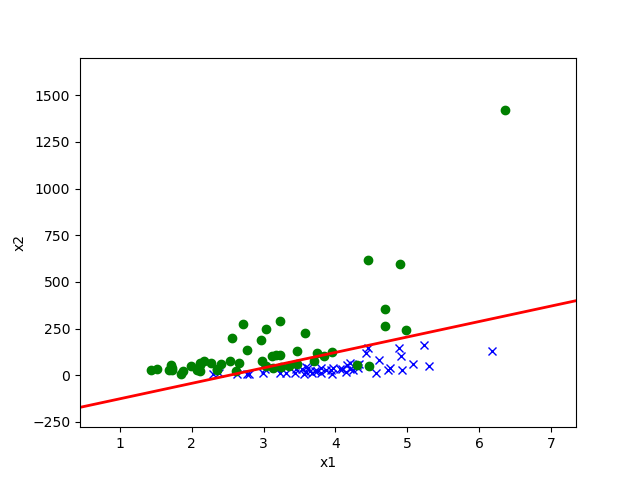
\includegraphics[width=\linewidth]{pics/p01b_pred_1.txt.png}
        \subcaption{Logistic Regression on Dataset 1}
    \end{subfigure}
    \begin{subfigure}[b]{0.5\linewidth}
        \centering
        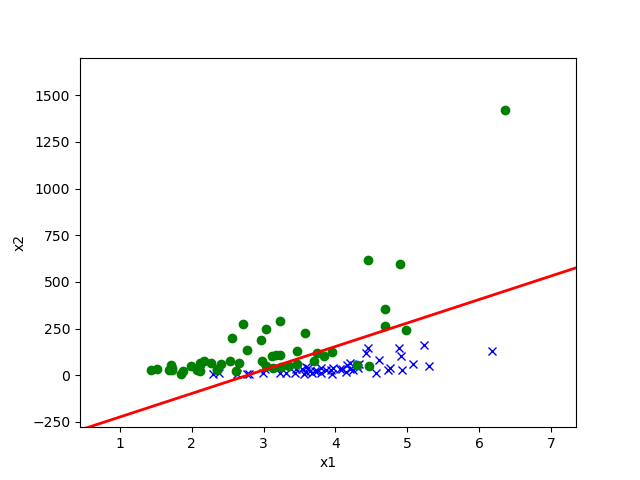
\includegraphics[width=\linewidth]{pics/p01e_pred_1.txt.png}
        \subcaption{GDA on Dataset 1}
    \end{subfigure}

\end{figure}

\end{answer}
} \fi

	\clearpage
\item \subquestionpoints{5}
Repeat the steps in part (f) for Dataset 2. On which dataset does GDA seem to
perform worse than logistic regression? Why might this be the case?

\ifnum\solutions=1{
  \begin{answer}

\end{answer}

}\fi

	\clearpage
\item \points{3 extra credit} For the dataset where GDA performed worse in
parts (f) and (g), can you find a transformation of the $x^{(i)}$'s such
that GDA performs significantly better? What is this transformation?

\ifnum\solutions=1{
  \begin{answer}
\end{answer}

}\fi

\end{enumerate}
